\section{Introduction}

A \textit{social network} is the collection of \textit{actors} and the \textit{relations} between each pair of actors.  
A mathematical graph is a natural way to represent a network, with actors as nodes and the relations between them as the edges (see Figure \ref{fig1}).  %However, beyond some shared terminology, there is little usage of graph theory in social network analysis.  
Publication of social network related papers in the social science literature has grown massively over the last forty years as the field has garnered increasing attention across different social and behavioral science disciplines \citep{Knoke:2007, Carrington:2005}.  \citet{Wasserman:1994} attribute this to researchers' realization that the network perspective, by focusing on the relational ties between interacting units, creates a new structured framework with which to answer social behavioral science research questions.

\begin{figure} 
\begin{center} 
\scalebox{.6}{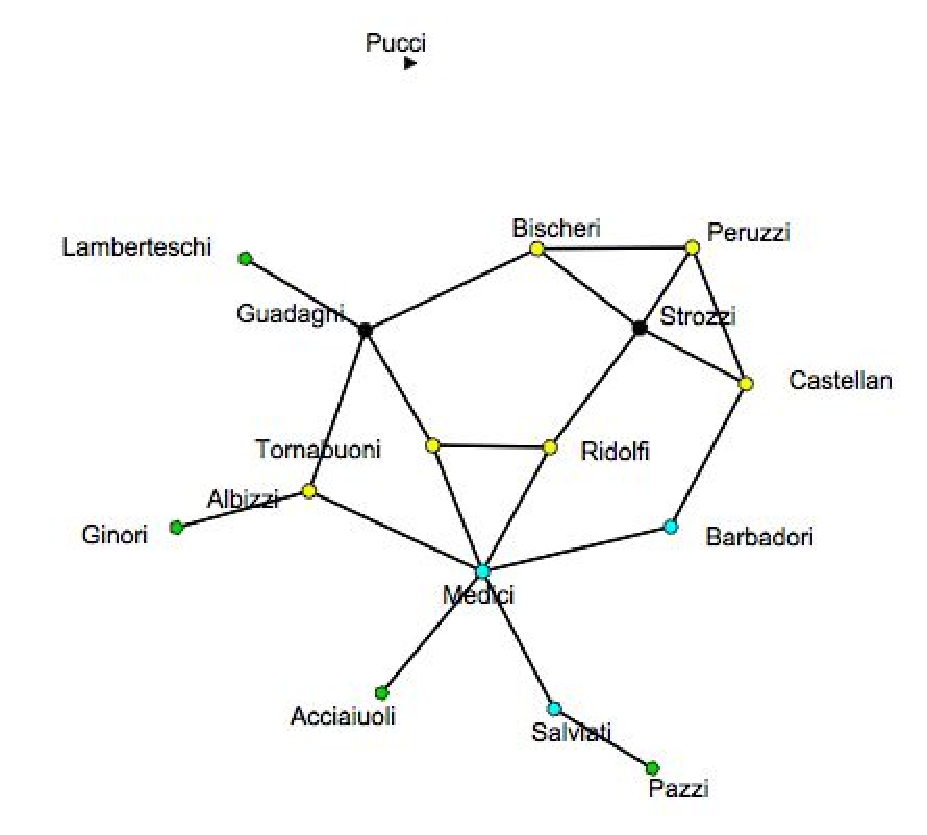
\includegraphics{myfigures/medici.eps}}
\end{center} 
\caption{Padgett's Renaissance Florentine family marriage network (1994).  Data set in \texttt{statnet} \citep{statnet:R}.} 
\label{fig1} 
\end{figure} 


  Although problems from sociology provide much of the motivations for social network analysis, network models can be applied to problems in a broad range of disciplines including political science, communications, marketing, and epidemiology.  Actors often represent individuals but they may also represent entities like nation-states, computers, or corporations.  The relation that connects actors is often friendship or actor $i$ ``liking" actor $j$ when the actors are individuals, but the tie can be any kind of relation such as a business transaction or the Internet connectedness between computers.  

Researchers have developed many \textit{descriptive} statistics that capture characteristics of an social network.  For example, the number of ties going to a particular actor is one measure of that actor's prestige in that network \citep{Wasserman:1994}.  Such statistics characterize properties of an observed network.  

In contrast, a statistical model can help us think about the distribution of possible unobserved outcomes.  It may illuminate local selection forces that shape the global structure of the network \citep{introp*, ergm}.  A good model will allow us to simulate a new network that retains some essential properties of the original network \citep{statnet}.  The challenge is to capture the interdependent nature of tie formation; in most social network environments, the chance that a tie will form between two actors $A$ and $B$ may be influenced by how likely a tie is to form between actors $B$ and $C$.  If we are looking at a monogamous marriage data set between individuals, the probability of Ross and Darrah being married will be highly affected by how likely Darrah and Nick are to be married!  Treating the ties as the response variable, the lack of independence between the ties marks a significant departure from the classical regression model where responses are treated as independent and raises the need for more complex models.  These complex models in turn require more sophisticated methods to calibrate them to the network data, a process that is still in its developmental stages as is evidenced by the stream of recent research on this topic \citep{Hunter:2006, Handcock:2006, recentp*, Morris:2008, Duijn:2009}.

In this proposal, we review the existing methods of finding parameter estimators for network models, including maximum pseudolikelihood estimators (MPLEs) and Markov chain Monte Carlo maximum likelihood estimators (MCMCMLEs).  We then present a simple algorithm that converges to the maximum likelihood estimators (MLEs) of a full exponential family distribution, the probability model underlying most social network models.  Unlike standard line search algorithms, our algorithm utilizes first derivative information only, evaluating neither the likelihood function itself nor derivatives of higher order than first which are expensive to compute when Markov chain Monte Carlo evaluation is used.


%%%%%%%%%%%%%%%%% SECTION %%%%%%%%%%%
\section{Introduction to Modeling}
Social networks are typically modeled as a random network represented by a matrix $Y$, an $n \times n$ matrix where $n$ is the number of actors.
Each entry $Y_{ij}$ in the random matrix $Y$ is a random variable representing a relation from actor $i$ to actor $j$, such that:
\[
	Y_{ij} = 
	\begin{cases}
		1 & \text{if a relationship exists \textit{from} actor $i$ \textit{to} actor $j$ (notation: $i \to j$)}\\
		0 & \text{otherwise}
	\end{cases}
	\
\]
where $i$ and $j$ take values in $1, \ldots, n$, $i \neq j$, for a network with $n$ actors.  Note that $Y_{ij}$ take only values of $0$ or $1$, reflecting our restriction on networks to those with dichotomous relations, that is, the relation between a pair of actors is either present or absent.  In addition, we do not allow the possibility of $i \to i$ and always denote $Y_{ii} = 0$.  In the special case that $Y_{ij} = Y_{ji}$ and thus the matrix $Y$ is symmetric, the network is referred to as a \textit{undirected} network or graph.  A network is \textit{directed} if it is not undirected.  

The exponential family random graph model (ERGM) commonly used in the network literature for $Y$ is as follows:
\begin{align}
	P_{\eta}(Y=y) &= \frac{ \exp(\eta^T g(y) ) }{ \kappa( \eta) } \qquad y \in \YY, \label{E:ERGM}
\end{align}
where $g(y)$ is a $q$-vector of statistics, $\eta$ is a $q$-vector of parameters, $\YY$ is the whole sample space of allowable networks which may contain $N = 2^{n(n-1)}$ networks if graphs are directed and $N = 2^{n(n-1)/2}$ if graphs are undirected, and $\kappa(\eta)$ is the normalizing constant such that
\begin{align*}
   \kappa(\eta) &= \int \exp [ \eta^T g(x) ] \, d \mu(x) %\label{E:kappa}
\end{align*}
where $\mu$ is a counting measure on $\YY$.  Thus an ERGM is a discrete exponential family distribution in canonical form \citep{tpe} and we will rely on many of the properties of exponential families.

We define the \textit{natural} parameter space $\Xi$ for $\eta$,
\begin{align}
   \Xi &= \{ \eta \in \RR^q : \kappa(\eta) < \infty \}.  \label{E:paramspace}
\end{align}
We find it also useful to define
\begin{align*}
	c(\eta) &= \log \kappa(\eta).
\end{align*}

Then our ERGM model \eqref{E:ERGM} can alternatively be expressed as 
\begin{align*}
	P_{\eta}(Y=y) &= \exp \left (\eta^T g(y) - c(\eta) \right ) \qquad y \in \YY.
\end{align*}
Also, we will frequently work with the log-likelihood of \eqref{E:ERGM}, that is,
\begin{align}
	\ell( \eta ) = \eta^T g(y) - c( \eta). \label{E:loglike}
\end{align}
%%%%%%%%% MAXIMUM ENTROPY APPROACH?
MAXIMUM ENTROPY?  \citep{Geyer:1992}[p. 666]

%%%%%%%%% NETWORK STATISTICS
A researcher specifies the statistics that compose the vector $g(y)$ in \eqref{E:ERGM} depending on what tie configurations he is concerned with modeling.  For example, a sociologist may be interested in the propensity for individuals to form reciprocal relations, where ties exist $i \to j$ and $j \to i$, or transitive relations, where ties exist $i \to j$, $j \to k$, $i \to k$.  The vector $g(y)$ can then be defined to be 
\begin{align*}
g(y) = \left ( \sum_{i<j} Y_{ij}Y_{ji}, \sum_{i \neq j \neq k} Y_{ij}Y_{jk}Y_{ik} \right )  
\end{align*}
where the components count the number of reciprocal and transitive tie configurations, respectively.  \citet{Wasserman:1996, Pattison:1999, logit, introp*} explore various network statistics that one might include in the vector $g(y)$.  

We will not discuss the merits or purpose of all the different network statistics here; what is important is that these statistics can be transparently calculated for a given network and the inclusion of them in $g(y)$, along with their parameters, allows the model to calculate probabilities of the presence of their associated tie formations.  In the works cited above, the researchers' primary consideration in defining a network statistic is to find a tie configuration that is of particular relevance to a problem.  For example, since reciprocity of ``liking" between individuals is commonly observed in friendship networks, it would be sensible to include a statistic for the number of reciprocal ties \citep{Holland:1981}.  Such a model, with parameters appropriately calibrated to a friendship network, might then generate networks that exhibit a significantly different number of reciprocal ties than would be expected in a uniformly random network.

%\begin{figure}[!h]
%\centering
%\scalebox{1}{\includegraphics{tableofstats.eps}}
%\caption{Table of some commonly used basic network statistics.}
%\label{fig2} 
%\end{figure}
%%%%%% TABLE OF COMMONLY USED NETWORK STATISTICS

  \citet{Handcock:2006, Hunter:2006, recentp*} continue the work of defining new network statistics but focus on the sensibility of the distributions generated from the specified models rather than just the scientific significance of certain tie configurations.  A complete description of network statistics is in \citet{Morris:2008}.  In addition, the issue of model selection between competing models has not been addressed though \citet{GOF} have begun making strides in this area.  Both of these areas are active area of research.

Finally, it should be noted that information about a particular node, say the gender for an individual, can be incorporated as \textit{covariate} data by allowing $g(y)$ to depend on a node-specific covariate matrix $X$.  Thus we may write $g(y, X)$ in place of $g(y)$ in \eqref{E:ERGM}.  We will continue to use $g(y)$ here for simplicity.


\section{Examples of ERGMs}

\subsection{Erd\H{o}s-R\'{e}nyi model}
The simplest example of an exponential random graph is the Erd\H{o}s-R\'{e}nyi model, also referred to as a Bernoulli network model, which assumes that all actors form a relation to other actors with the same probability, $p$ \citep{Wasserman:1994, ergm}.  The ERGM can be expressed as
\begin{align*}
	P_{\eta}(Y=y) &= \frac{ \exp(\eta g(y) ) }{ \kappa( \eta) } \qquad y \in \YY, 
\end{align*}
where the only statistic is a count of the number of edges for the network so that
\begin{align*}
%	g(y) = \frac{1}{N}\sum_{i \neq j} y_{ij},
	g(y) = \sum_{i \neq j} y_{ij}
\end{align*}
and the probability of a tie formation between any pair of actors is
\begin{align*}
	p = \frac{\exp(\eta)}{1+ \exp(\eta)}.
\end{align*}
As such, the $Y_{ij}$ are mutually independent of one another.  
The MLE of $\eta$ can found by taking the logit of the fraction of ties that are present in the data set, 
\begin{align*}
	\etaMLE = \logit \left ( \frac{\sum_{i \neq j} y_{ij}}{ N } \right )
\end{align*}
where $N = n(n-1)$, the number of possible ties in a network with $n$ actors.  The MLE for $\eta$ is easily calculated from the observed data but the independence assumption is too unrealistic for all but the simplest of cases; usually, a researcher is interested in the different probabilities of tie formations between actors.

\subsection{The $p_1$ Model}
\citet{Holland:1981} made advances in relaxing this independence assumption  with their $p_1$ model.  They focused on two empirical observations from sociometric studies:
\begin{itemize}
\item Reciprocation: there tend to be a ``surplus" of mutual relationships in network data sets compared to a uniform distribution of directed relationships.
\item Stars: some individuals attract a surplus of choices compared to a uniform distribution of directed relationships.
\end{itemize}
\citeauthor{Holland:1981} then constructed a family of distributions with parameters to control the probability of observing different numbers of mutual relationships and stars.  
Focusing on the \textit{dyad}, the set of a pair of actors and the possible relations between them, as the basic building block, they proposed the following model:
\[
	P( Y = y ) = \frac{1}{ K( \rho, \theta, \{ \alpha_i \}, \{\beta_j \} )}\exp \left \{  \rho m(y) + \theta y_{++} + \sum_i \alpha_i y_{i+} +  \sum_j \beta_j y_{+j}\right \}
\]
subject to $\sum_i \alpha_i = \sum_j \beta_j = 0$, where
\begin{align*}
	\rho &= \text{``force of reciprocation" or mutuality parameter}\\
	m(y) &= \sum_{i \neq j} y_{ij}y_{ji}, \quad \text{number of mutual relationships in $y$}\\
	\theta &= \text{``density" or overall choice effect parameter}\\
	y_{++} &= \sum_{i \neq j} y_{ij}, \quad  \text{total number of relations in $y$}\\
	\alpha_i &= \text{``productivity" or ``expansiveness" effect parameter for node $i$}\\
	y_{i+} &= \sum_{j} y_{ij}, \quad  \text{``out-degree" for node $i$ in $y$}\\
	\beta_j &= \text{``attractiveness" or ``popularity" effect parameter for node $j$} \\
	y_{+j} &= \sum_{i} y_{ij}, \quad  \text{``in-degree" for node $j$ in $y$}\\
	K &= \text{normalizing constant}
\end{align*}

By defining new dyad random variables, $D_{ij} = (Y_{ij}, Y_{ji} )$, \citeauthor{Holland:1981}  show that with some algebraic manipulation the form of the model above can be viewed as a log-linear model with independent dyad random variables, $D_{ij}$.  This makes it possible to use a logistic regression to calculate MLEs of the parameters.

The statistical independence at the dyad level, however, means that this model will not capture triangular tie configurations in which dyads are dependent.  Also, to reduce the number of parameters, the model assume $\rho_{ij} = \rho$, meaning that the tendency towards reciprocity is assumed to be the same across all actors.  Similarly, the model assumes that $\theta$ is the same across all actors.  This example illustrates how the parameter estimation methodology limits the scope of the model and what types of behavior it can capture.  

\subsection{Markov Graph Model}
\citet{Frank:1986} relax the independence assumption further with the implementation of \textit{Markov dependence} in which two dyads are independent, conditional on the rest of the graph, when they do not share a node.  The model use only three configurations in an \textit{undirected}, expressed as:
\[
	P( Y = y ) = \frac{1}{K( \theta, \sigma, \tau)}\exp \left \{ \theta L + \sigma S + \tau T	\right \} 
	\]
where
\begin{align*}
	\theta &= 		\text{Edge parameter} \\
	L &= 		\text{Number of edges} \\
	\sigma &= \text{2-Star parameter, propensity for individuals to have connections with two actors} \\
	S &= \text{Number of 2-stars ($i \leftrightarrow j$, $i \leftrightarrow k$) }\\
	\tau	&= \text{Triangle parameter, represents clustering} \\
	T &= \text{Number of triangles ($i \leftrightarrow j$, $j \leftrightarrow k$, $i \leftrightarrow k$)} \\
\end{align*}
None of the above parameters have subscript indices, reflecting the simplification from a \textit{homogeneity} assumption where parameters are equated if the configurations are the same ignoring the labels on the nodes (also called \textit{isomorphic} configurations.  In fact, this is the same simplification Holland and Leinhardt employ for the $\rho$ parameter in their $p1$ model.)  

The model is the first to break dyad independence, made possible by \citeauthor{Frank:1986}' methods of parameter estimation.  In particular, \citeauthor{Frank:1986} run Markov chain Monte Carlo simulations of the model at multiple values for a parameter to determine which fits the data best.  The authors also get maximum pseudolikelihood estimators (MPLE) obtained from a standard logistic regression and observe that the MPLEs are close to those from their simulations.  We will discuss the maximum pseudolikelihood methodology in the next section.  However, it may be noted here that it is this simplification of parameter estimation that has perpetuated the evolution of the network model to its general ERGM form \eqref{E:ERGM} that we consider in this paper.  
%More recent work has shown that this model with the exhibits problems with \textit{degeneracy} in which a model fit with parameters set to MLEs will generate only graphs that are empty or complete \citep{Handcock:Degeneracy}.  


%%%%%%%%%%%%%%%%% SECTION %%%%%%%%%%%

\section{Parameter Estimation}
Parameter estimation in statistical models is typically done through the method of maximum likelihood estimation in which values for the parameters, called maximum likelihood estimators (MLEs), that make the observed data most likely for the model are calculated.  Unfortunately, maximum likelihood for exponential families can be difficult for our model \eqref{E:ERGM} because the the normalizing constant $\kappa(\theta)$, a function of the very parameters we are trying to estimate, can be prohibitively expensive to evaluate.  For a directed network with $n$ actors, there are $N=2^{n(n-1)}$ different possible networks in our state space $\YY$, a huge number for even a moderate sized $n$.  It is for this reason that researchers like \citet{Holland:1981} made the restrictive assumptions of dyad independence for the $p_1$ model to enable the use of a logistic regression.  In this section we discuss the maximum pseudolikelihood and Markov chain Monte Carlo methods that have been developed to obtain estimators for the model parameters. 



\subsection{Maximum Pseudolikelihood method}
As mentioned in the previous section, \citet{Frank:1986} introduced the application of the maximum pseudolikelihood method, a method used in lattice systems \citep{Besag:1974}, to social network models.  \citet{Strauss:1990} further justify the use of maximum pseudolikelihood estimators (MPLE) as reasonable approximations for MLEs in social network models.  \citet{Wasserman:1996, Pattison:1999, logit} grasp the significance of this simplification and broaden the scope of network models to allow for any combination of network statistics, constrained only by the number of parameters. 

The method of maximum pseudolikelihood finds the values for the parameters that maximize the \textit{pseudolikelihood} or pseudo-loglikelihood functions for the given data set, which can be constructed from the distributions of a single tie, $Y_{ij}$, conditional on the rest of the network, which we will abbreviate as ``rest".  The conditional distribution of $Y_{ij} | \textrm{rest}$ is a Bernoulli distribution with log odds:
\begin{align}
	\log \left \{ \frac{P( Y_{ij} =1 | \textrm{rest} ) }{ P( Y_{ij} =0 | \textrm{rest} ) } \right \} = \eta^T \Delta(g(y))_{ij}, \label{E:logodds}
\end{align}
where we define the vector of \textit{change statistics}, $\Delta(g(y))_{ij}$, to be
%which is the change in $g(y)$ when $y_{ij}$ changes from 0 to 1 while the rest of the network remains the same,  
\begin{align*}
	\Delta(g(y))_{ij} = g(y_{ij}^+) - g(y_{ij}^-)
\end{align*}
where $y_{ij}^+$ and $y_{ij}^-$ represent networks with $y_{ij} = 1$ or $y_{ij} = 0$, respectively, while leaving the rest of the network as $y$.  Thus $\Delta(g(y))_{ij}$ is the change in $g(y)$ when $y_{ij}$ changes from 0 to 1.

The pseudolikelihood is constructed from \eqref{E:logodds} by assuming that the $Y_{ij}$ are in fact mutually independent, that is, 
\begin{align*}
	P( Y_{ij} =1 | \textrm{rest} ) = P( Y_{ij} =1 ).
\end{align*}
With this independence assumption, \eqref{E:logodds} is exactly the setup for a logistic regression through which we can get the estimates of $\eta$, called the maximum pseudolikelihood estimators, or MPLEs.  In the case where the dyads are in fact independent, the MPLEs will equal the MLEs.  \citet{Strauss:1990} show that in many cases with dyad dependence, MPLE still yield reasonable approximations of the true MLEs for social network models.  However, \citet{Geyer:1992, Snijders:2002, Duijn:2009} demonstrate that MPLEs can produce very misleading results, and social network software packages such as \texttt{statnet} in the \texttt{R} platform now use MLE methods rather than MPLE \citep{statnet:R}.  

\subsection{Markov chain Monte Carlo methods}
\citet{Geyer:1992, Corander:1998, Snijders:2002} developed Markov chain Monte Carlo (MCMC) methods to approximate the MLE of an exponential family.  Of these, \citeauthor{Geyer:1992}'s MCMCMLE method appears to be most commonly implemented in the literature and software \citep{Hunter:2006, Handcock:2006, ergm, statnet, GOF}.  

Rather than maximizing the log-likelihood \eqref{E:loglike},
\[	\ell(\eta ) = \eta ^T g(y) - c(\eta) \]
with respect to $\eta$, \citeauthor{Geyer:1992} fix $\eta^0$ at a known value and look to maximize the log of the likelihood ratio\footnote{In fact, $r(\eta, \eta^0)$ is also a log-likelihood.  The addition to $\ell (\eta)$ of an arbitrary function of data that does not contain the parameter $\eta$ will still observe the definition of a log-likelihood.}, $r( \eta, \eta^0 )$.
\begin{align}
 r( \eta, \eta^0 ) &= \ell( \eta ) - \ell( \eta^0 ) \notag \\ 
					&= ( \eta - \eta^0)^T g(y) - \log \left [ \exp \{ c(\eta) - c(\eta^0) \} \right ]. \label{E:r}
\end{align}
The approach then focuses on approximating the ratio of normalizing constants, $\frac{ \exp \{c(\eta) \} }{ \exp \{c(\eta^0) \} }$.  The value of $\eta$ that maximizes the approximation of $r( \eta, \eta^0 )$ is then a good estimate of the MLE when it exists.  This can be seen by starting with the normalizing constant,
\begin{align*}
	\exp \{c(\eta) \} &= \int \exp\{\eta^Tg(x)\} \, d\mu(x).
\end{align*}
The ratio of normalizing constants is then
\begin{align*}
	\exp\{ c(\eta) - c(\eta^0) \} &= \frac{ \int \exp\{\eta^Tg(x)\} \, d\mu(x) }{ \exp\{ c(\eta^0) \} } \\
	&= \frac{ \int \exp\{( \eta - \eta^0)^T g(x) + (\eta^0)^Tg(x)\}\, d\mu(x)  }{ \exp\{ c(\eta^0) \} } \\
	&= \int \exp\{( \eta - \eta^0)^T g(x) \} \frac{ \exp \{(\eta^0)^T g(x)\} }{ \exp\{ c(\eta^0) \}  } \, d\mu(x)\\
	&= \E_{\eta^0} \left [ \exp\{ ( \eta - \eta^0)^T g(Y)  \} \right ].
\end{align*}

By the Markov chain strong law of large numbers (or Birkhoff ergodic theorem), this expectation can be approximated by the sample mean for large sample size,
\begin{align*}
	&\approx \frac{1}{m} \sum_{i=1}^{m}\exp \{ ( \eta - \eta^0)^Tg(Y_i) \}
\end{align*}
where $Y_1, \ldots, Y_m$ are draws from the exponential family distribution with parameter $\eta^0$.  This sample can be generated using Markov chain Monte Carlo method such as a Metropolis algorithm.

Thus, $r( \eta, \eta^0 )$ can be approximated by
\begin{align}
\hat{r}_m( \eta, \eta^0 ) &= ( \eta - \eta^0)^Tg(y) - \log \left [ \frac{1}{m} \sum_{i=1}^{m} \exp \{ ( \eta - \eta^0)^Tg(Y_i)\} \right ] \label{E:r_hat}
\end{align}
and 
\begin{align*}
	\hat{r}_m( \eta, \eta^0 ) \to r( \eta, \eta^0 ) \text{ a.s. as $m \to \infty$}.
\end{align*}

If we call the maximizer of \eqref{E:r_hat} $\hat{\eta}_m$ and assume that the MLE $\etaMLE$ exists, \citeauthor{Geyer:1992} show that 
\begin{align*}
\hat{\eta}_m \to \etaMLE \quad a.s.
\end{align*}
 whenever the Markov chain is ergodic. 

In practice, \citeauthor{Geyer:1992} recognize that ``enormous" Monte Carlo sample sizes may be necessary and that best results are obtained when $\eta^0$ is near $\etaMLE$---a condition that of course cannot be checked since $\etaMLE$ is unknown!  In addition, \citeauthor{Geyer:1992} recommend iterating the algorithm several times, where each successive value will be closer to $\etaMLE$ than the previous.  At the time of this writing, the MCMCMLE routine in \texttt{statnet} uses by default 10,000 Monte Carlo samples and a maximum of three iterations \citep{statnet:R}, using the MPLE as the initial value for $\eta^0$.  We follow up with an example presented by \citet{ergm} in \texttt{statnet} in which the MCMCMLE procedure can fail.

\vspace*{0.2in}

\textbf{Sampson's Monastery Data set}

\begin{figure} 
\begin{center} 
\scalebox{.6}{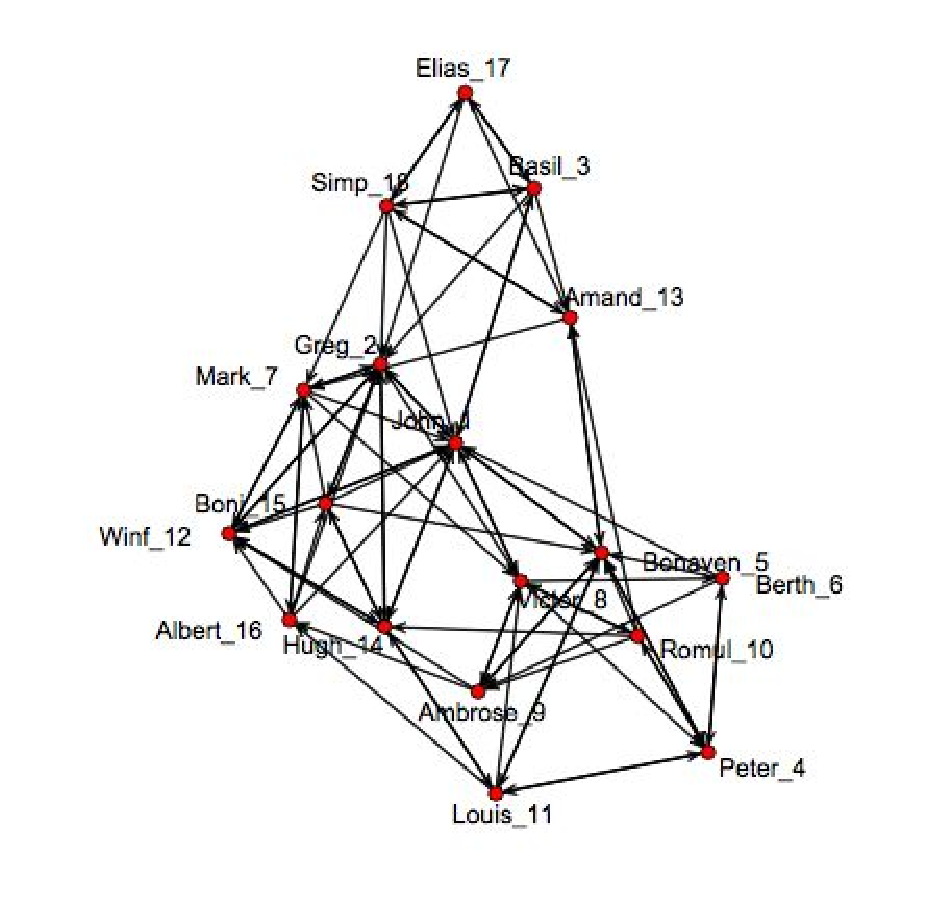
\includegraphics{myfigures/samplike.eps}}
\end{center} 
\caption{Sampson's monastery affinity network (1969).} 
\label{fig-samplike} 
\end{figure} 

\citeauthor{ergm} illustrate the practical difficulty associated with a poor initial value in the MCMCMLE algorithm with Sampson's monastery data set, a standard data set in the social network literature which we depict in Figure \ref{fig-samplike}.  The network is directed with 18 actors and 88 ties present out of $18(17)=306$ possible ties.  For this data set \citeauthor{ergm} use the simple Erd\H{o}s-R\'{e}nyi model described earlier, with the network statistic $g(y)$ equal to the total number of edges present, so $g(y_{obs}) = 88$.  The true MLE is equal to $\logit(88/306) = -0.9072$.  When $\eta^0$ is chosen to be $1$, however, \citeauthor{ergm} demonstrate that the algorithm will fail in a single iteration.  With $\eta=1$, the model describes that each of the 306 possible edges will occur independently with probability $p = \frac{1}{1+e^{-\eta}} = \frac{1}{1+e^{-1}} = 0.731$.  The problem arises from the fact that this is a high probability relative to the observed data set, which suggests a much smaller probability of tie formation of $88/306= 0.288$.  In fact, the probability of obtaining $g(Y) < g(y_{obs})=88$ is close to zero at $2.3 \times 10^{-59}$, where $g(Y)$ are generated from a binomial distribution with $n=306$, $p =0.731$.  The MCMCMLE algorithm looks to maximize the approximated log likelihood ratio \eqref{E:r_hat}, but if the MC sample is unable to generate $g(Y)< g(y_{obs})$, \eqref{E:r_hat} will not have a maximizer since the function will not have a point where the derivative is zero (see upper solid line in Figure \ref{F:bad eta}).  The problem is not present when an initial value close to the true MLE like $\eta^0 = -1$ is used (lower solid line in Figure \ref{F:bad eta}).  With the default three iterations in the \texttt{statnet} software, the algorithm gets to $\eta = -0.364$, but with 10 iterations it arrives at the MLE.

\begin{figure} 
\begin{center} 
\scalebox{.8}{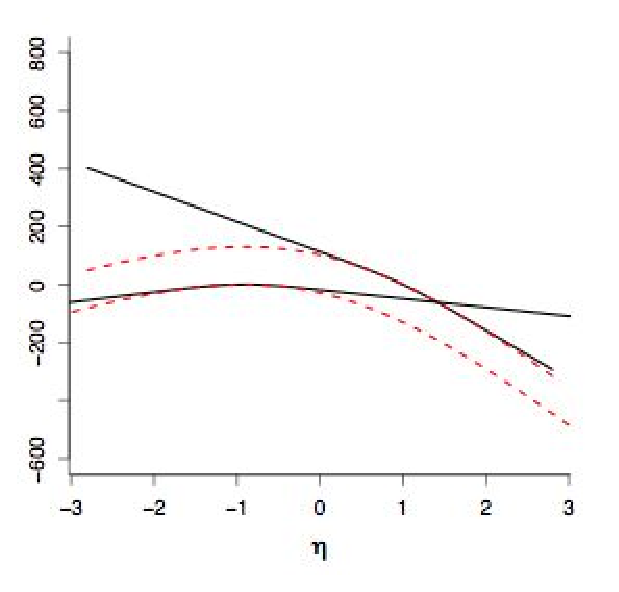
\includegraphics{myfigures/bad_eta.eps}}
\end{center} 
\caption{Log likelihood ratios for different values of $\eta$ for the Sampson Monastery data set.  Dotted lines are exact log likelihood ratios, solid lines are the approximation by \eqref{E:r_hat}.  Upper solid and dotted lines correspond to $\eta^0 = 1$, lower lines correspond to $\eta^0 = -1$.  The upper solid line, the approximate log likelihood ratio with $\eta^0 = 1$, has no maximizing value of $\eta$ \citep{ergm}.} 
\end{figure} 

%\begin{align*}
%\hat{r}_m( \eta, \eta^0 ) &= ( \eta - \eta^0)^Tg(y) - \log \left [ \frac{1}{m} \sum_{i=1}^{m} \exp \{ ( \eta - \eta^0)^Tg(Y_i)\} \right ] 
%\end{align*}
